\documentclass[11pt]{article}
\usepackage[cm]{fullpage}
\usepackage{graphicx}
\usepackage{caption}
\usepackage{subcaption}
\usepackage[section]{placeins}
\usepackage{float}
\usepackage{amsmath}
\usepackage{multicol}

\setlength{\columnsep}{1cm}

\title{S1336 - Project 2}
\author{Erik Weilow}

\newcommand{\doublefigure}[2]{
\begin{figure}[H]
  \centering
  \begin{minipage}{0.45\textwidth}
    \centering
    \includegraphics[width=\textwidth]{#1}
  \end{minipage}
  \begin{minipage}{0.45\textwidth}
    \centering
    \includegraphics[width=\textwidth]{#2}
  \end{minipage}
\end{figure}
}
\newcommand{\singlefigure}[1]{
\begin{figure}[H]
  \centering
  \begin{minipage}{0.4\textwidth}
    \centering
    \includegraphics[width=\textwidth]{#1}
  \end{minipage}
\end{figure}
}

\begin{document}
\maketitle
\newpage

\section*{2.1}

\subsection*{Effects of rounding errors}
\doublefigure{./plots/2_1/r06.png}{./plots/2_1/r091.png}

It can be concluded that when $r < r_\infty$, rounding doesn't have much of an effect on the system.

When $r > r_\infty$, rounding does however have an effect on the system.

\section*{2.2}

If settling for $n=200$, we can use the following formula to calculate $\lambda$:
$$
\lambda = \frac{1}{n} \sum_{i=0}^{i=n-1}{\text{log}\left| \frac{\Delta x_{i+1}}{\Delta x_i}\right|}
$$

This can be done numerically by solving the system, for many values of $r$.

\subsection*{The Lyapunov exponent for a population model}
\singlefigure{./plots/2_2/study.png}
We see that for $0.76 < r < r_\infty$, when the system isn't chaotic, the sign of $\lambda$ is positive.
Effects of rounding doesn't affect $\lambda$ unless $r > r_\infty$.

\subsection*{The dependence on initial value}
\begin{figure}[H]
  \centering
  \begin{minipage}{0.8\textwidth}
    \centering
    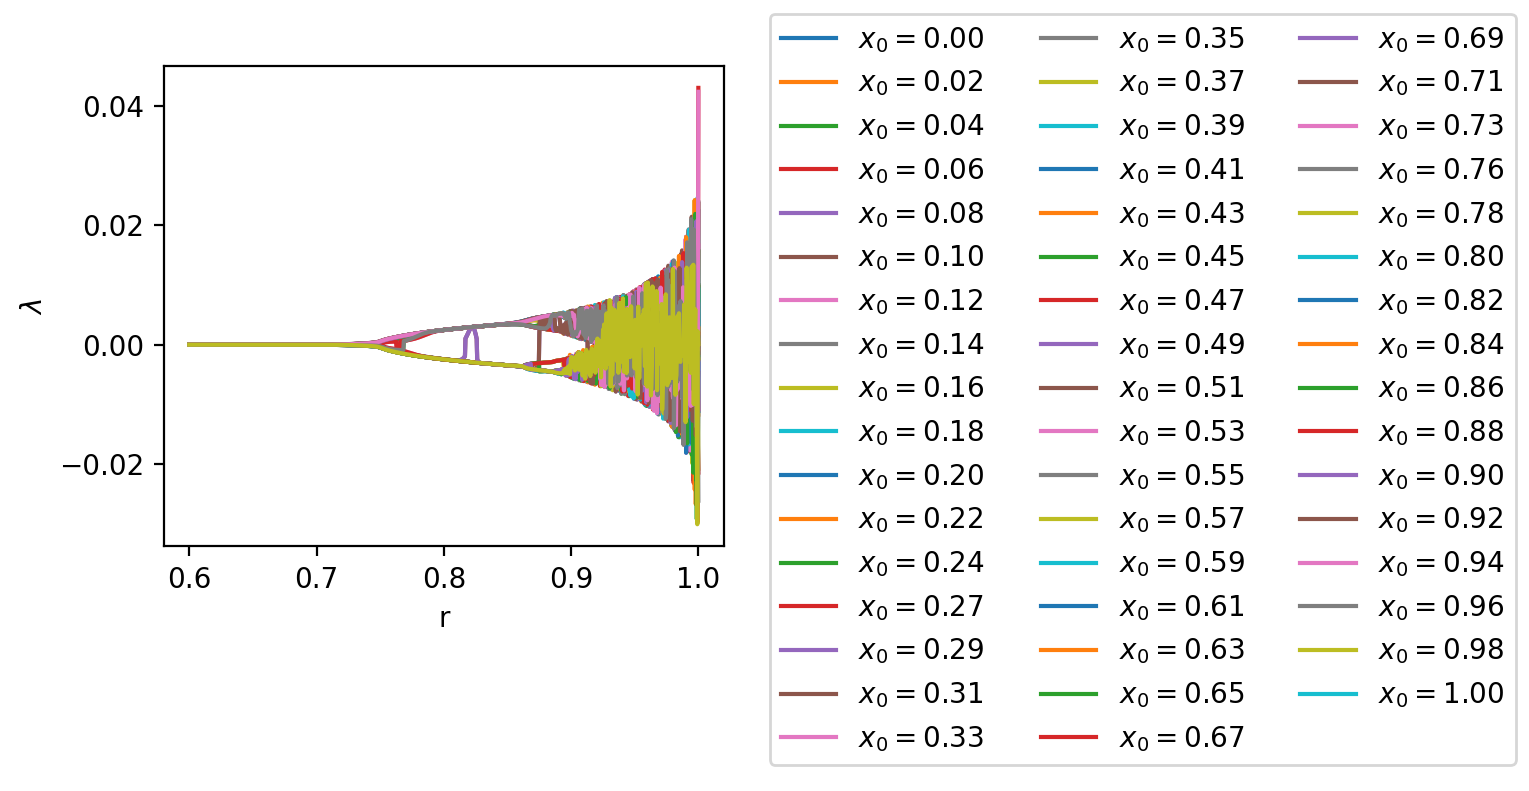
\includegraphics[width=\textwidth]{./plots/2_2/dependence.png}
  \end{minipage}
\end{figure}
In this plot, we see that selecting different $x_0$ has an effect on the calculation of $\lambda$.
For $r < 0.76$, it's clear that the system is non-chaotic since $\lambda$ is strictly equal to 0.
For approximately $0.76 < r < 0.87$, $\lambda$ is either positive or negative depending on the initial value.
It then takes on many values, incredibly dependent on $x_0$.

\section*{2.3}

\subsection*{Lorenz attractor}
To figure out which parts of space get attracted in to the basin of the Lorenz attractor, trajectories for different starting conditions randomly sampled on the interval
$$
x(0) \in (-1000, 1000), \quad
y(0) \in (-1000, 1000), \quad
z(0) \in (-1000, 1000) \\
$$
are computed. 

The time averaged "radius" is calculated for each trajectory:
$$
r = \frac{1}{n} \sum_{i=0}^n{\sqrt{x{(i \Delta t)}^2 + y{(i \Delta t)}^2 + z{(i \Delta t)}^2}}
$$

25 CPU hours later, for a time step of $\Delta t = 0.00008$ and a time boundary of $0 < t < 150$, the following histogram can be plotted:
\singlefigure{./plots/2_3/histo.png}

It shows that for all (roughly 2500) computed trajectories, they all average to within a distance 60 from $x = 0, y = 0, z = 0$.
We can thus conclude that it's very unlikely that a solution doesn't get attracted into the basin.

It's also interesting to note that the distribution is starting to look like a normal distribution. This could be investigated further in the future and left as an excercise for the reader. 
\section*{2.4}

\subsection*{Sensitivity to initial values}
\doublefigure{./plots/2_4/solution.png}{./plots/2_4/difference.png}

The right plot shows the "distance" between the solutions at each time $t$.
It can be seen that even for a small difference in initial value ($0.01$), the solutions differ much after some time.

\newpage


\section*{2.5}

\begin{multicols}{2}
\subsection*{Chaos or not?}
\singlefigure{./plots/2_5/study.png}
We see that a solution starting in $x(0) = 10, y(0) = 0, z(0) = 0$ has an average of about $z = 28$, coincidentally the same number as the value for $r$ given in the task.
 
\columnbreak
\singlefigure{./plots/2_5/peaks.png}
It's clear that the ratio $\frac{z_{m+1}}{z_m}$ isn't strictly greater than unity.
\end{multicols}


\end{document}